本系統的架構如圖片。系統總共由以下元素組成:

\begin{itemize}
  \item 文件 Corpus $D$。其中一份文件 $d_i\in D$ 代表一本書或是一個開放式課程。
  \item 每份文件 $d_i\in D$ 是一個序列 $d_i = (s_{i,1},\dots,s_{i,m_i})$,
        代表書的目錄或是開放式課程的課表。$s_{i,j}$ 是個字串,為書本目錄的
        一個 section 或課程進度表的一個項目。
  \item \textproc{Search} 函數。給定一串搜尋關鍵字 $k$,\textproc{Search}$(k)$
        是所有包含這些關鍵字的文件的集合。
  \item \textproc{GenerateKeyword} 函數。給定文件子集 $D'\subset D$,
        \textproc{GenerateKeyword}$(D')$ 會回傳是文件子集 $D'$ 中的重要關鍵字,
        並會依據重要性做 ranking。
  \item \textproc{GenerateFlow} 函數。給定文件子集 $D'\subset D$,
        \textproc{GenerateFlow}$(D')$ 是將 $D'$ 中文件的目錄或課表適當地 cluster
        與 ranking 形成的整合目錄。
\end{itemize}

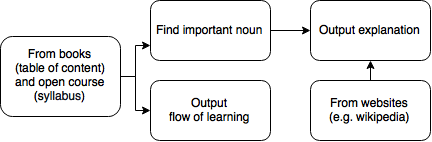
\includegraphics[scale=0.55]{./diagram.png}

